\chapter{早终止加速算法}
\label{cha:algorithm}

\section{基于树剪枝的早终止算法}

\subsection{原始算法}

在 \ref{sec:current-status} 部分曾提到,K Choi和SH Park等人在HEVC上针对四叉树划分过程提出了优化算法,
该算法使用率失真代价作为衡量标准,在满足一定条件时对四叉树进行剪枝,从而节省了子节点的计算量,以达到加速的
目的。该算法是清晰而简洁的,作为跨视频编码标准来移植的对象是十分合适的,因此,笔者选定该算法作为移植的最初
对象。

% 可以考虑加入,通过减少CU深度来降低复杂度的说明

首先对原算法做介绍。原算法针对H.265标准提出,与AV1有所不同,在四叉编码树的组织上,H.265中使用CU、PU、TU来
实现对编码单元我的组织,PU和TU是在CU划分的基础上进一步划分而来的,因此,我们不妨仅关注对CU的划分优化。原文中
提出的一种较为直接的思路是,当当前CU节点的代价低于该节点子节点的代价时,我们就不必再对子树进行进一步的处理,
公式化的表述如 \ref{eq-algrithm-hevc-rdcost} 所示。

\begin{equation}
\label{eq-algrithm-hevc-rdcost}
RDCost(CU_t) < \sum_{i=0}^3 RDCost(CU^i_{t-1})
\end{equation}

% 展开解释RDCost?

这里,$CU_t$是当前节点,$CU^i_{t-1}$为子节点,$RDCost$为率失真代价。这一方法问题在于子树的代价必须是已知的,这一要求使得计算复杂度
的减少程度是有限的。因此,为了更大限度地减少计算复杂度,原文提出了新的剪枝公式 \ref{eq-algrithm-origin}。

\begin{equation}
\label{eq-algrithm-origin}
(\mathop{m'} =  \mathop{argmin}\limits_{m \in Mode} RDCost(CU_t | PU=m)) \le Threshold 
\end{equation}

这里,Mode表示H.265中预测模式的集合,而$\mathop{m'}$则是为当前CU深度选择的预测模式,Threshold的值由Mode
决定。即新的剪枝公式通过为不同的预测模式定制不同的阈值,并将节点代价与该阈值进行比较进行剪枝,从而避免了子树
代价必须已知的条件。根据上述分析,绘制原算法的流程图如 \ref{fig:algorithm-h265-flowchart} 所示。需要说明的
是,该流程图只是一个将主要过程及分支点抽出后的示意图,实际情况更为复杂,例如叶子节点的处理以及非四分模式最优
时递归也会停止等情况。

\begin{figure}[H] % use float package if you want it here
  \centering
  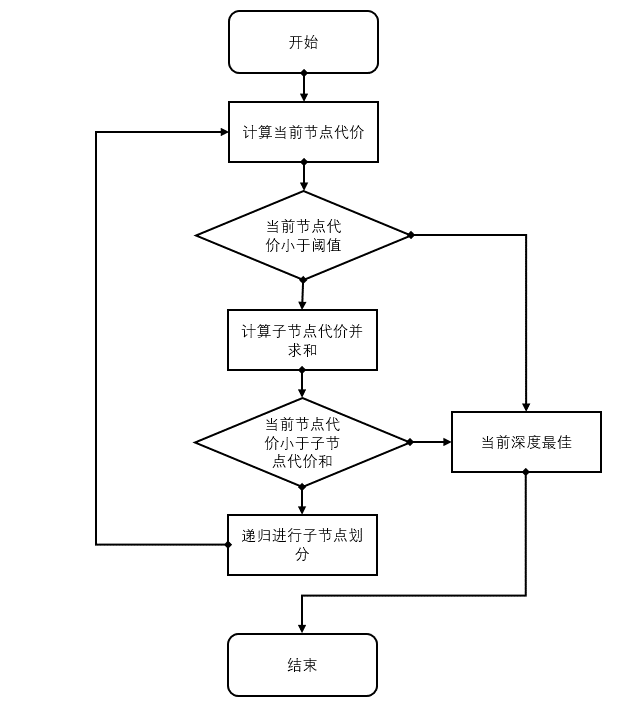
\includegraphics[width = 0.6\textwidth]{algorithm-h265-flowchart}
  \caption{H.265树剪枝早终止算法流程图}
  \label{fig:algorithm-h265-flowchart}
\end{figure}

\subsection{原始算法成果}

原论文中,编码的表现以 $\Delta Bitrate[ (B_{PRO} - B_{REF})/B_{REF} * 100 ]$ 和 $ \Delta PSNR(P_{PRO} - P_{REF})$ 
来衡量,并且时间的减少以 $ \Delta Time[ (T_{PRO} - T_{REF})/T_{REF} * 100 ]$ 来衡量。所选用的测试视频为H.265上所使用
的五类典型测试用视频。

在以可忽略不计的画面质量降低以及比特率损失为代价的前提下,相较于HM3.0编码器,该方法可以提供最差28\%、最好58 \%的时间缩减,
平均来看,该方法能有效节省编码时间约40\%。这是十分出色的成果,在移植算法时,该方法是十分清晰的,因此有着很高的可移植性,
尽管AV1标准与H.265有诸多不同,但如此优秀的成果在移植后,我们可以期望其有着不错的表现。

\section{移植到AV1上的树剪枝算法}

\subsection{原算法的缺陷}

尽管原算法有着简明的形式和优异的表现,但观察剪枝的核心条件 \ref{eq-algrithm-origin} 不难发现,Threshold的值对于剪枝至关
重要,该阈值完全决定了当前节点的子节点代价是否需要计算。然而,原论文中仅指出Threshold的值应根据预测模式进行选取,而该值具体
是多少、应当如何确定,原文并没有给出详细的策略。因此,在移植时,针对单一模式确定Threshold的值是十分困难的。甚至H.265中,
所需要应对的模式仅有 $\{ SKIP, Inter2Nx2N, Inter2NxN, InterNx2N, InterNxN \} $ 五种,而在AV1中,除去常规的上述几种外,
还引入了如 \ref{fig:coding-av1-mode} 所示的T型划分和水平/垂直四分,这使得Threshold的数量增多,测定难度进一步加大。

\subsection{阈值测定的尝试}

较大的阈值测定难度并不妨碍笔者对Threshold值的推断作出一些初步的努力,笔者以park\_joy\_90p\_8\_420这一AV1上的典型测试用
视频进行探究,设定编码后视频的比特率为200,对各节点RDCost的值做一些统计。被统计节点共5166个,这些节点中,RDCost最小值为
68,393、最大值1,829,405,236、平均值为23,431,775、中位数为5,683,608。可以看到,RDCost的极差是非常大的。更直观的分布示意图
如 \ref{fig:algorithm-rdcost-distribution} 所示,不难看出,RDCost主要分布在值较小的区域内。

\begin{figure}[H]
  \centering%
  \begin{subfigure}{0.43\textwidth}
    \centering
    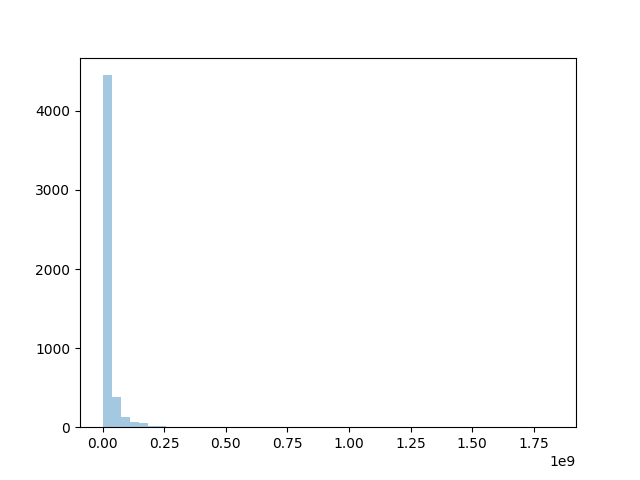
\includegraphics[height = 4.5cm]{algorithm-rdcost-distribution}
    \caption{park\_joy视频RDCost分布直方图}
  \end{subfigure}%
  \hspace{2em}%
  \begin{subfigure}{0.43\textwidth}
    \centering
    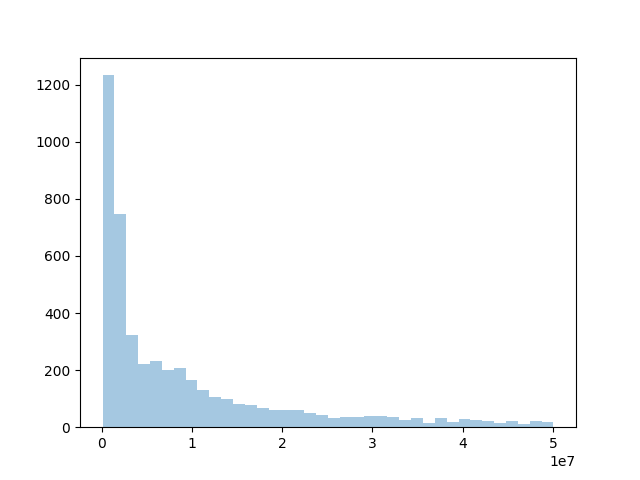
\includegraphics[height = 4.5cm]{algorithm-rdcost-distribution-500}
    \caption{去除500个最大值后的直方图}
  \end{subfigure}
  \caption{park\_joy视频RDCost分布}
  \label{fig:algorithm-rdcost-distribution}
\end{figure}

同样是对park\_joy\_90p\_8\_420视频限定比特率为200时,在测定RDCost的同时,笔者还记录了当时节点所存储的各个模式中的最佳RDCost
的值,并做统计分析。在最佳RDCost的统计中,最小值581、最大值2,077,618,636、平均值24,020,189、中位数3,490,404。直方图如 
\ref{fig:algorithm-best-rdcost-distribution} 所示,可以看到最佳RDCost的分布趋势与RDCost一致,都集中在数值较小的范围内,
且平均来看数值更小。

\begin{figure}[H]
  \centering%
  \begin{subfigure}{0.43\textwidth}
    \centering
    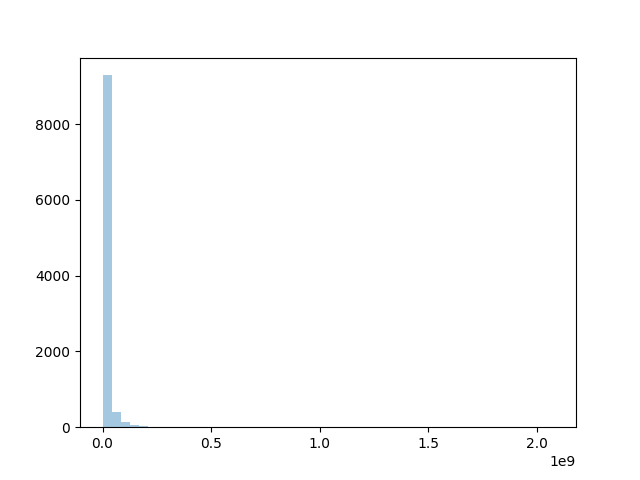
\includegraphics[height = 4.5cm]{algorithm-best-rdcost-distribution}
    \caption{park\_joy视频最佳RDCost分布}
  \end{subfigure}%
  \hspace{2em}%
  \begin{subfigure}{0.43\textwidth}
    \centering
    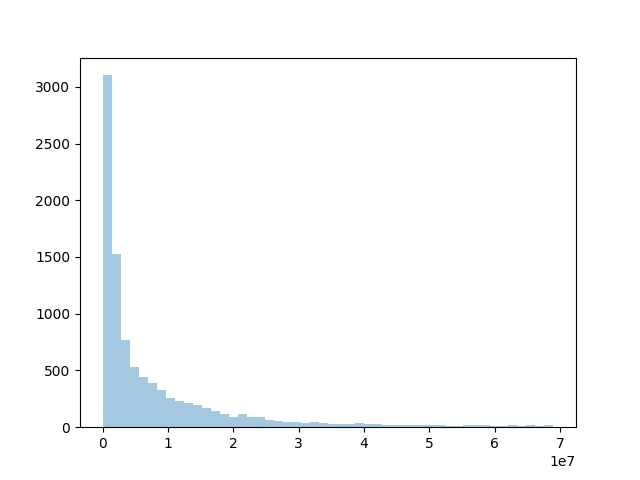
\includegraphics[height = 4.5cm]{algorithm-best-rdcost-distribution-500}
    \caption{去除500个最大值后的分布}
  \end{subfigure}
  \caption{park\_joy视频最佳RDCost分布}
  \label{fig:algorithm-best-rdcost-distribution}
\end{figure}

由上述分析可以看出,确实可以通过选择一个值作为Threshold来过滤掉RDCost大于该值的节点划分模式,从而实现加速。例如,可以得知
80\%的最佳RDCost小于16,037,601,因此我们可以较为保守地选取该值作为Threshold,当当前节点所对应模式的RDCost大于该值时,
该模式不大可能是该节点的最优划分方式。

% 换一个视频
当然,上述的结论仅是针对park\_joy\_90p\_8\_420这一个视频成立的。笔者又对另一个AV1测试用视频miss\_am\_qcif进行了测试,
当限定比特率为200时,得到的分布结果如 \ref{fig:algorithm-rdcost-distribution-miss} 图所示。

\begin{figure}[H]
  \centering%
  \begin{subfigure}{0.43\textwidth}
    \centering
    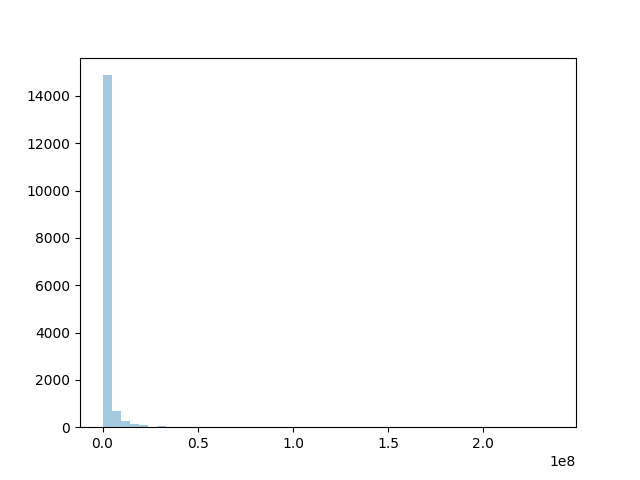
\includegraphics[height = 4.5cm]{algorithm-rdcost-distribution-miss}
    \caption{miss\_am\_qcif视频RDCost分布}
  \end{subfigure}%
  \hspace{2em}%
  \begin{subfigure}{0.43\textwidth}
    \centering
    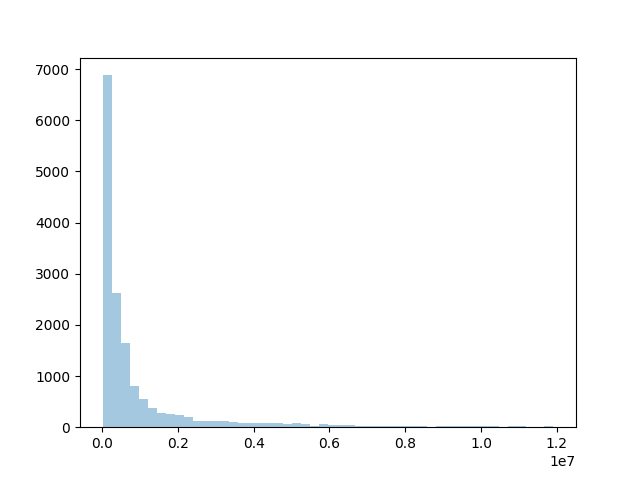
\includegraphics[height = 4.5cm]{algorithm-rdcost-distribution-miss-500}
    \caption{去除500个最大值后的分布}
  \end{subfigure}
  \caption{miss\_am\_qcif视频RDCost分布}
  \label{fig:algorithm-rdcost-distribution-miss}
\end{figure}

对测试用视频miss\_am\_qcif编码过程中各节点的RDCost分布进行统计,得到其最小值15754、最大值236,766,106、
平均值1,905,168、中位数349,230。显然,这与park\_joy视频所得到的数值差了一个数量级,若仍以之前针对park\_joy
提出的值作为Threshold,则该阈值将几乎无法做出有效的筛选。

由上述两个个例的测试结果,不难发现在AV1编码标准下,针对不同的视频,RDCost的分布差距可能是巨大的,因此,针对每种划分模式
提出一个合理的、适用于绝大多数视频的Threshold是十分困难的。因此,在时间精力有限的前提下,笔者放弃了通过对大量视频测试筛选
Threshold的思路,退而求其次,使用效果不那么好、但确定性强、基于与子节点代价和比较的剪枝策略。

\subsection{AV1中的RDCost}

\subsection{移植后的算法}

\section{加权树剪枝早终止算法}